\let\negmedspace\undefined
\let\negthickspace\undefined
\documentclass[journal]{IEEEtran}
\usepackage[a5paper, margin=10mm, onecolumn]{geometry}
\usepackage{lmodern} % Ensure lmodern is loaded for pdflatex
\usepackage{tfrupee} % Include tfrupee package

\setlength{\headheight}{1cm} % Set the height of the header box
\setlength{\headsep}{0mm}     % Set the distance between the header box and the top of the text

\usepackage{gvv-book}
\usepackage{gvv}
\usepackage{cite}
\usepackage{amsmath,amssymb,amsfonts,amsthm}
\usepackage{algorithmic}
\usepackage{graphicx}
\usepackage{textcomp}
\usepackage{xcolor}
\usepackage{txfonts}
\usepackage{listings}
\usepackage{enumitem}
\usepackage{mathtools}
\usepackage{gensymb}
\usepackage{comment}
\usepackage[breaklinks=true]{hyperref}
\usepackage{tkz-euclide} 
\usepackage{listings}
\def\inputGnumericTable{}                                 
\usepackage[latin1]{inputenc}                                
\usepackage{color}                                            
\usepackage{array}                                            
\usepackage{longtable}                                       
\usepackage{calc}                                             
\usepackage{multirow}                                         
\usepackage{hhline}                                           
\usepackage{ifthen}                                           
\usepackage{lscape}

\begin{document}
	
	\bibliographystyle{IEEEtran}
	\vspace{3cm}
	
	\title{12.9.ex.19}
	\author{EE24BTECH11030 - KEDARANANDA}
	% \maketitle
	% \newpage
	% \bigskip
	{\let\newpage\relax\maketitle}
	
	\renewcommand{\thefigure}{\theenumi}
	\renewcommand{\thetable}{\theenumi}
	\setlength{\intextsep}{10pt} % Space between text and floats
	\textbf{Question:}
	
	Solve the differential equation:
	
	$y' = y + \cos x$
	
	\textbf{Solution:}
	
	\textbf{Theoretical solution:}
	
	The given differential equation is a first-order linear ordinary differential equation. Let $y(0) = c_1$. By the definition of the Laplace transform,
	
	$\mathcal{L}(f(t)) = \int_0^\infty e^{-st} f(t) \, dt$
	
	Some used properties of the Laplace transform include:
	\begin{align}
		\mathcal{L}(f'(t)) &= s\mathcal{L}(f(t)) - f(0) \\
		\mathcal{L}(cf(t)) &= c\mathcal{L}(f(t)) \\
		\mathcal{L}(e^{at}f(t)) &= F(s - a), \quad \text{where } F(s) = \mathcal{L}(f(t)) \\
		\mathcal{L}(\cos x) &= \frac{s}{s^2 + 1}
	\end{align}
	
	\textbf{Applying the Laplace transform to the given differential equation:}
	
	$y' - y = \cos x$
	
	Take the Laplace transform on both sides:
	
	\begin{align}
		\mathcal{L}(y') - \mathcal{L}(y) &= \mathcal{L}(\cos x)
	\end{align}
	
	Using the properties of the Laplace transform:
	
	\begin{align}
		(s\mathcal{L}(y) - y(0)) - \mathcal{L}(y) &= \frac{s}{s^2 + 1}
	\end{align}
	
	Let $\mathcal{L}(y) = Y(s)$. Substituting $y(0) = c_1$, we get:
	
	\begin{align}
		sY(s) - c_1 - Y(s) &= \frac{s}{s^2 + 1}
	\end{align}
	
	Simplify:
	
	\begin{align}
		(s - 1)Y(s) &= c_1 + \frac{s}{s^2 + 1} \\
		Y(s) &= \frac{c_1}{s - 1} + \frac{s}{(s^2 + 1)(s - 1)}
	\end{align}
	
	\textbf{Partial fraction decomposition:}
	
	For $\frac{s}{(s^2 + 1)(s - 1)}$, decompose into:
	
	\begin{align}
		\frac{s}{(s^2 + 1)(s - 1)} &= \frac{A}{s - 1} + \frac{Bs + C}{s^2 + 1}
	\end{align}
	
	Solve for $A$, $B$, and $C$ by equating numerators:
	
	\begin{align}
		s &= A(s^2 + 1) + (Bs + C)(s - 1)
	\end{align}
	
	
	
	Equating coefficients:
	\begin{align}
		A + B &= 0 \quad \text{(coefficient of $s^2$)} \\
		-B + C &= 1 \quad \text{(coefficient of $s$)} \\
		A - C &= 0 \quad \text{(constant term)}
	\end{align}
	
	
	The partial fraction decomposition becomes:
	
	\begin{align}
		\frac{s}{(s^2 + 1)(s - 1)} &= \frac{\frac{1}{2}}{s - 1} + \frac{-\frac{1}{2}s + \frac{1}{2}}{s^2 + 1}
	\end{align}
	
	\textbf{Rewrite $Y(s)$:}
	
	\begin{align}
		Y(s) &= \frac{c_1}{s - 1} + \frac{\frac{1}{2}}{s - 1} + \frac{-\frac{1}{2}s + \frac{1}{2}}{s^2 + 1}
	\end{align}
	
	Combine terms:
	
	\begin{align}
		Y(s) &= \frac{c_1 + \frac{1}{2}}{s - 1} - \frac{\frac{1}{2}s}{s^2 + 1} + \frac{\frac{1}{2}}{s^2 + 1}
	\end{align}
	
	\textbf{Take the inverse Laplace transform:}
	
	Using the properties of the Laplace transform:
	\begin{align}
		\mathcal{L}^{-1}\left(\frac{1}{s - 1}\right) &= e^t \\
		\mathcal{L}^{-1}\left(\frac{s}{s^2 + 1}\right) &= \cos t \\
		\mathcal{L}^{-1}\left(\frac{1}{s^2 + 1}\right) &= \sin t
	\end{align}
	
	Apply the inverse transform to each term:
	
	\begin{align}
		y(t) &= \left(c_1 + \frac{1}{2}\right)e^t - \frac{1}{2}\cos t + \frac{1}{2}\sin t
	\end{align}
	
	\textbf{Final solution:}
	
	\begin{align}
		y(x) &= \left(c_1 + \frac{1}{2}\right)e^x - \frac{1}{2}\cos x + \frac{1}{2}\sin x
	\end{align}
	
	We use the bilinear $z$-transform:
	\begin{align}
		s &= \frac{2}{T} \frac{1 - z^{-1}}{1 + z^{-1}}.
	\end{align}
	
	Step 1: Substitute and Simplify Each Term
	
	First Term: $ \frac{c_1 + \frac{1}{2}}{s - 1} $
	Substitute $s = \frac{2}{T} \frac{1 - z^{-1}}{1 + z^{-1}}$:
	\begin{align}
		\frac{c_1 + \frac{1}{2}}{s - 1} &= \frac{c_1 + \frac{1}{2}}{\frac{2}{T} \frac{1 - z^{-1}}{1 + z^{-1}} - 1}.
	\end{align}
	
	Simplify the denominator:
	\begin{align}
		\frac{2}{T} \frac{1 - z^{-1}}{1 + z^{-1}} - 1 &= \frac{\frac{2}{T} (1 - z^{-1}) - (1 + z^{-1})}{1 + z^{-1}}.
	\end{align}
	
	Thus:
	\begin{align}
		\frac{c_1 + \frac{1}{2}}{s - 1} &= (c_1 + \frac{1}{2}) \cdot \frac{1 + z^{-1}}{\frac{2}{T} - 1 - \left(\frac{2}{T} + 1\right)z^{-1}}.
	\end{align}
	
	Second Term: $ -\frac{\frac{1}{2}s}{s^2 + 1} $
	Substitute $s = \frac{2}{T} \frac{1 - z^{-1}}{1 + z^{-1}}$:
	\begin{align}
		-\frac{\frac{1}{2}s}{s^2 + 1} &= -\frac{\frac{1}{2} \cdot \frac{2}{T} \frac{1 - z^{-1}}{1 + z^{-1}}}{\left(\frac{2}{T} \frac{1 - z^{-1}}{1 + z^{-1}}\right)^2 + 1}.
	\end{align}
	Simplify:
	\begin{align}
		-\frac{\frac{1}{2}s}{s^2 + 1} &= -\frac{\frac{1}{2} \cdot \frac{2}{T} \frac{1 - z^{-1}}{1 + z^{-1}}}{\left(\frac{2}{T} \frac{1 - z^{-1}}{1 + z^{-1}}\right)^2 + 1} \\
		&= -\frac{\frac{1}{T} (1 - z^{-1})}{\frac{\left(\frac{2}{T}\right)^2 (1 - z^{-1})^2}{(1 + z^{-1})^2} + 1} \\
		&= -\frac{\frac{1}{T} (1 - z^{-1})(1 + z^{-1})^2}{\left(\frac{2}{T}\right)^2 (1 - z^{-1})^2 + (1 + z^{-1})^2}.
	\end{align}
	
	Third Term: $ \frac{\frac{1}{2}}{s^2 + 1} $
	Substitute $s = \frac{2}{T} \frac{1 - z^{-1}}{1 + z^{-1}}$:
	\begin{align}
		\frac{\frac{1}{2}}{s^2 + 1} &= \frac{\frac{1}{2}}{\frac{\left(\frac{2}{T} \frac{1 - z^{-1}}{1 + z^{-1}}\right)^2 + 1}{(1 + z^{-1})^2}} \\
		&= \frac{\frac{1}{2} (1 + z^{-1})^2}{\left(\frac{2}{T}\right)^2 (1 - z^{-1})^2 + (1 + z^{-1})^2}.
	\end{align}
	
	Step 2: Combine Terms
	The total $Y(z)$ is:
	\begin{align}
		(c_1 + \frac{1}{2}) \cdot \frac{1 + z^{-1}}{\frac{2}{T} - 1 - \left(\frac{2}{T} + 1\right)z^{-1}} 
		- \frac{\frac{1}{T} (1 - z^{-1})}{\left(\frac{2}{T}\right)^2 (1 - z^{-1})^2 + (1 + z^{-1})^2} 
		+ \frac{\frac{1}{2} (1 + z^{-1})^2}{\left(\frac{2}{T}\right)^2 (1 - z^{-1})^2 + (1 + z^{-1})^2}
	\end{align}
	\textbf{Computational Solution Bilinear:(sim2)}
	% Step 2
	\begin{align}
		\left(\frac{2}{T}\right)^2 \left(1 - z^{-1}\right)^2 + \left(1 + z^{-1}\right)^2
		\Bigg)^{-1} 
		\Bigg[
		\left(\frac{2}{T} - 1\right) - \left(\frac{2}{T} + 1\right)z^{-1} 
		\Bigg] Y(z) \nonumber \\
		&= f(z^{-1}, z^{-2}, z^{-3}) + c
	\end{align}
	% Step 3
	\begin{align}
		\left(\frac{4}{T^2} + 1\right) + \left(2 - \frac{8}{T^2}\right)z^{-1} + \left(\frac{4}{T^2} + 1\right)z^{-2} 
		\Bigg) \Bigg(\frac{2}{T} - 1 - \left(\frac{2}{T} + 1\right)z^{-1}\Bigg) Y(z) \nonumber \\
		&= f(z^{-1}, z^{-2}, z^{-3}) + c
	\end{align}
	
	
	% Step 4
	\begin{align}
		\left(a + bz^{-1} + cz^{-2}\right) \left(d + ez^{-1}\right) Y(z) = f(z^{-1}, z^{-2}, z^{-3}) + c
	\end{align}
	
	% Step 5
	\begin{align}
		adY(z) + (ae+bd)z^{-1}Y(z) + (cd+be)z^{-2}Y(z) + ce z^{-3}Y(z) \nonumber \\
		&= f(z^{-1}, z^{-2}, z^{-3}) + c
	\end{align}
	
	% Step 6
	\begin{align}
		\text{where } 
		a = \left(\frac{4}{T^2}+1\right), \, 
		b = \left(2-\frac{8}{T^2}\right), \, 
		c = \left(\frac{4}{T^2}+1\right), \, \nonumber 
		d = \frac{2}{T}-1, \, 
		e = -\left(\frac{2}{T}+1\right)
	\end{align}
	
	% Step 7
	\begin{align}
		&\rightarrow 
		adz^{3}Y(z) + (ae+bd)z^{2}Y(z) + (cd+be)z^{1}Y(z) + ceY(z) \nonumber \\
		&= f'(z^{1}, z^{2}, z^{3}) + c
	\end{align}
	
	% Step 8
	\begin{align}
		&\rightarrow 
		ady[n+3] + (ae+bd)y[n+2] + (cd+be)y[n+1] + cey[n] \nonumber \\
		&= f''(\delta[n], \delta[n+1], \delta[n+2], \delta[n+3])
	\end{align}
	
	% Step 9
	\begin{align}
		\text{Given: } y[0] = c_{1}, \, y[1] &= y[0] + h y'[0]
	\end{align}
	
	% Step 10
	\begin{align}
		y[1] &= c_{1} + h(1+a)
	\end{align}
	
	% Step 11
	\begin{align}
		y[2] &= y[1] + h(y'[1])
	\end{align}
	
	% Step 12
	\begin{align}
		y[2] &= y[1] + h(y[1] + \cos(h))
	\end{align}
	
	% Step 13
	\begin{align}
		y[3] &= y[2] + h(y[2] + \cos(2h))
	\end{align}
	
	% Step 14
	\begin{align}
		n \geq 1 \rightarrow \delta[n], \delta[n+1], \delta[n+2], \delta[n+3] &= 0
	\end{align}
	
	% Step 15
	\begin{align}
		\text{Difference equation: } 
		y[n+3] &= -\frac{1}{ad} \left[(ae+bd)y[n+2] + (cd+be)y[n+1] + cey[n]\right]
	\end{align}
	\textbf{Computational Solution: Trapezoid Method:(sim1)}
	
	\subsection*{Step 1: Transform the DE into a First-Order System}
	
	The given differential equation is already in first-order form:
	$\frac{dy}{dx} = y + \cos x$.
	
	Let:
	$y = y_1$, so $\frac{dy_1}{dx} = y_1 + \cos x$.
	
	\subsection*{Step 2: Apply the Trapezoidal Rule}
	
	Using the Trapezoidal Rule, the equation can be written as:
	\begin{align}
		y_{n+1} - y_n &= \frac{h}{2} \big( (y_n + \cos x_n) + (y_{n+1} + \cos x_{n+1}) \big),
	\end{align}
	where $h$ is the step size, $y_n$ is the value of $y$ at $x_n$, and $y_{n+1}$ is the value of $y$ at $x_{n+1} = x_n + h$.
	
	\subsection*{Step 3: Solve for $y_{n+1}$}
	
	Rearranging Equation (1) to isolate $y_{n+1}$:
	\begin{align}
		y_{n+1} - \frac{h}{2} y_{n+1} &= y_n + \frac{h}{2} (y_n + \cos x_n + \cos x_{n+1}), \\
		y_{n+1} \big( 1 - \frac{h}{2} \big) &= y_n \big( 1 + \frac{h}{2} \big) + \frac{h}{2} (\cos x_n + \cos x_{n+1}), \\
		y_{n+1} &= \frac{y_n \big( 1 + \frac{h}{2} \big) + \frac{h}{2} (\cos x_n + \cos x_{n+1})}{1 - \frac{h}{2}}.
	\end{align}
	
	\subsection*{Step 4: Iterative Scheme}
	
	The final iterative formula is:
	\begin{align}
		y_{n+1} = \frac{y_n \big( 1 + \frac{h}{2} \big) + \frac{h}{2} (\cos x_n + \cos x_{n+1})}{1 - \frac{h}{2}}.
	\end{align}
	
	\subsection*{Step 5: Initial Conditions and Computation}
	
	Given the initial condition:
	$x_0 = 0$, $y_0 = 0$,
	and a chosen step size $h$, the values of $y_n$ can be iteratively computed for subsequent $x_n$.\\
	\begin{figure}[h!]
		\centering
		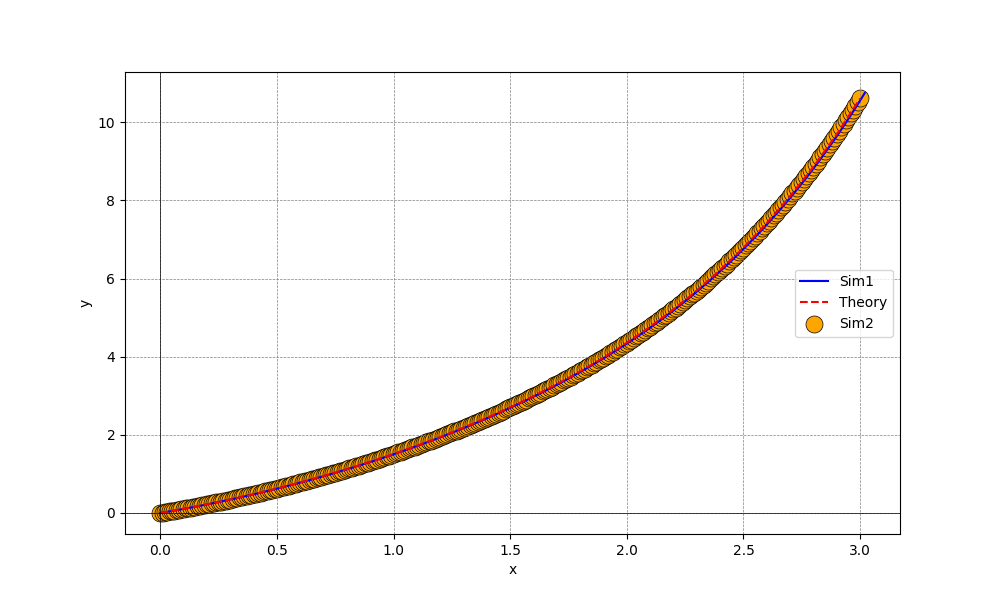
\includegraphics[width=0.7\columnwidth]{figs/Fig1.png}
		\caption{Here Sim-$1$ plot represents the plot given by Trapezoid Method, and Sim-$2$ which is given by Bilinear transform using the same value of $h$. This plot clearly shows the accuracy of the Bilinear transform method.}
		\label{label}
	\end{figure}
\end{document}